\documentclass[a4paper]{article}

\usepackage[english]{babel}
\usepackage[utf8]{inputenc}
\usepackage{amsmath}
\usepackage{graphicx}
\usepackage{algpseudocode}
\usepackage{algorithm}
%\usepackage[colorinlistoftodos]{todonotes}

\usepackage{amsmath}
\DeclareMathOperator*{\argmax}{arg\,max}
\DeclareMathOperator*{\argmin}{arg\,min}

\title{Elaborazione di dati tridimensionali: homework 2}

\author{Alberto Cenzato 1134707}

\date{\today}

\begin{document}
\maketitle

\begin{abstract}
Scopo di questo secondo homework era di familiarizzare con la libreria PCL. Sono stati svolti quattro esercizi di complessità crescente per approfondire diverse funzionalità di PCL: lettura di point cloud da file, lettura e visualizzazione dei valori contenuti nella point cloud, downsampling, calcolo di normali, keypoint e descrittori, registrazione di point cloud, people detection.
\end{abstract}

\section{Lab 1} \label{sec:lab1}
La prima esperienza era suddivisa in due esercizi. Nel primo lo scopo era di rimuovere dalla point cloud tutti i punti con $X > 0$ e colorare i rimanenti in blu. Nel secondo era necessario filtrare la point cloud facendo di fatto un downsample dell'immagine 3D con risoluzioni diverse per ogni quadrante del piano $X$-$Y$.

	\subsection{Algortimi utilizzati}
	Per quanto riguarda il primo esercizio non c'è molto da dire sugli algoritmi utilizzati. Infatti, per modificare il colore dei punti, è sufficiente iterare su tutti i punti, verificare se $X > 0$ e in caso affermativo copiare il punto in una nuova point cloud modificando il suo colore in blu. La nuova cloud sarà quindi definita $C' = \left\{p \in C | p.x > 0, p.b = 255 \right\}$.
	Per filtrare la point cloud invece è stata usata la classe di PCL \verb|VoxelGrid| che divide lo spazio 3D in voxel: tutti i punti all'interno di un voxel vengono approssimati col loro centroide. Modificando la dimensione degli spigoli dei voxel si ottiene un donwsample maggiore o minore.
	
	\subsection{Considerazioni}
	L'implementazione è stata piuttosto diretta a partire dai file di esempio forniti, sono state necessarie solo alcune modifiche. L'output del secondo esercizio è mostrato in figura \ref{fig:lab1} 
	
	\begin{figure}
		\centering
		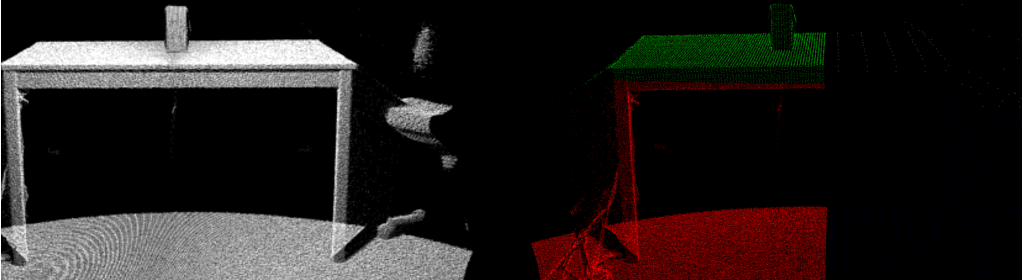
\includegraphics[width=1\textwidth]{images/lab1.png}
		\caption{\label{fig:lab1}Esempio di point cloud filtrata e colorata: a sinistra l'originale, a destra l'output.}
	\end{figure}


\section{Lab 2} \label{sec:lab2}
I due esercizi della seconda esperienza puntavano a calcolare le normali ad una superficie definita da una point cloud e ad utilizzare queste normali per il calcolo di features che possano essere caratteristiche e univoche per ogni punto.

	\subsection{Algortimi utilizzati}
	Il calcolo delle normali è stato fatto attraverso la classe di PCL \verb|NormalEstimationOMP|. \verb|NormalEstimationOMP| per ogni punto $p$ cerca i suoi vicini all'interno di una sfera di raggio $r$, questi vengono usati per stimare il piano $\pi^*$ che meglio approssima la superficie nel punto $p$; cioè si calcola 
	
	\begin{equation}
	\pi^* = \argmin_{\pi}{\sum_{x_i \in kNN(p)}{dist(x_i,\pi)}}
	\end{equation}
	
	\verb|NormalEstimationOMP| utilizza OpenMP per fornire un'implementazione multithread multipiattaforma. \\
	Vengono poi identificati i keypoint della point cloud, punti che per caratteristiche di posizione e/o colore rispetto ai loro vicini possono essere considerati salienti. Un buon keypoint detector dovrebbe essere invariante per traslazione, rotazione, scala e lumiosità, identificando sempre gli stessi keypoint indipendentemente dalle trasformazioni a cui viene sottoposta la point cloud. Per questo esercizio è stato scelto \verb|SIFT3D|, un'estensione di \verb|SIFT| in tre dimensioni, implementato dalla classe PCL \verb|SIFTKeypoint|. \\
	Una volta identificati i keypoint questi devono poter essere descritti o comparati in qualche modo. A questo scopo si utilizzano dei feature vector, cioè ad ogni keypoint viene assegnato un vettore caratteristico che identifica in modo univoco quel punto. Il contenuto dal vettore dipende dal feature descriptor utilizzato; per questo esercizio è stato usato \verb|Fast Point Feature Histogram|. L'algoritmo considera il keypoint e tutti i suoi vicini entro un raggio $r$; per ogni coppia dell'insieme vengono calcolati i tre angoli che definiscono l'orientazione reciproca delle due normali; infine crea un istogramma a partire dalle orientazioni di tutte le coppie. Il feature vector così estratto è invariante per rotazione e traslazione della point cloud.

	\subsection{Considerazioni}
	Il calcolo delle normali e l'estrazione delle features è piuttosto semplice grazie alle classi di PCL. La parte più lunga, come spesso accade con questi algoritmi, è la taratura dei parametri migliori per ottenere il risultato desiderato. Per \verb|SIFTKeypoint| sono stati usati \verb|min_scale = 0.01|, \verb|n_octaves = 3|, \verb|n_scales_per_octave = 4|, \verb|min_contrast = 0.001|. In figura \ref{fig:lab2} si possono vedere due esempi di descrittori calcolati con \verb|FPFHEstimationOMP|.
	
	\begin{figure}
		\centering
		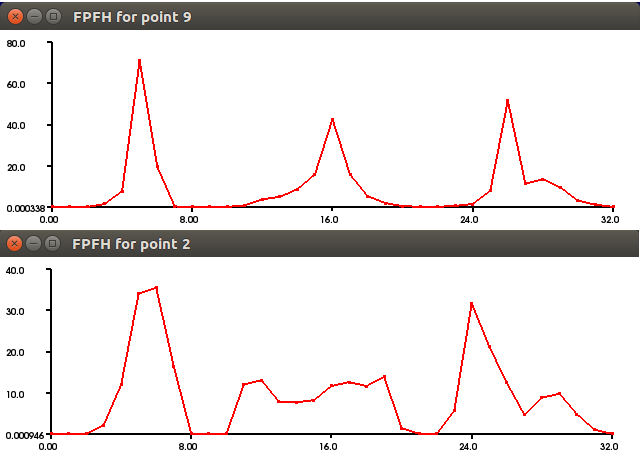
\includegraphics[width=1\textwidth]{images/lab2.png}
		\caption{\label{fig:lab2}Due esempi di descrittori FPFH per due keypoint diversi.}
	\end{figure}


\section{Lab 3} \label{sec:lab3}
La terza esperienza aveva lo scopo di registrare tra loro diverse point cloud della stessa scena. Nel primo esercizio due scansioni 3D di una stanza dovevano essere registrate tra loro. Le due cloud erano già grossolanamente allineate tra loro ed era necessario affinare la registrazione usando l'algoritmo ICP. Il secondo esercizio invece partiva da quattro point cloud dello stesso oggetto prese da angolazioni diverse ed è stato necessario calcolare le corrispondenze dei punti tra le varie point cloud per stimare una trasformazione approssimata che è stata poi affinata con ICP come nel primo esercizio.

	\subsection{Algortimi utilizzati}
	ICP (Iterative Closest Point) è un algoritmo pensato per allineare una point cloud \textit{source} $C_{s}$ con una point cloud \textit{target} $C_{t}$ minimizzando l'errore\footnote{La metrica dell'errore dipende dall'implementazione, un buon esempio è la somma quadratica delle distanze.}. Ad ogni iterazione l'algoritmo ad ogni punto di $C_{s}$ associa il più vicino punto in $C_{t}$, poi stima la rotazione $R$ e la traslazione $T$ che meglio allineano i punti in $C_{s}$ con quelli in  $C_{t}$. L'operazione viene ripetuta finché non si raggiunge una prefissata soglia inferiore sull'errore.

	\begin{equation}
	(R,T)^* = \argmin_{(R,T)}{Err(C_{t}, R*C_{s} + T)}
	\end{equation}
	
	dove $Err(C_1, C_2)$ potrebbe essere definito come:
	
	\begin{equation}
	Err(C_1, C_2) = \sum_{p_1 \in C_1, p_2 = \argmin_{p \in C_2}{dist(p_1, p)}}{dist(p_1,p_2)^2}
	\end{equation}
	
	Nel caso due point cloud non siano già ben allineate in partenza è necessario stimare una trasformazione approssimativa in modo da poter poi utilizzare ICP per l'allineamento finale.
	Questa operazione è stata svolta utilizzando la classe \verb|CorrespondenceEstimation|.

	\subsection{Considerazioni}
	Entrambi gli esercizi richiedevano un confronto tra due varianti dello stesso algoritmo. Nel primo si è confrontata la qualità della registrazione di due point cloud attraverso ICP utlizzando:
	\begin{itemize}
		\item una rappresentazione dei punti con le tre coordinate spaziali \verb|XYZ|;
		\item una rappresentazione \verb|XYZ| con l'aggiunta della curvatura della superficie;
	\end{itemize} 
	L'utilizzo della curvatura come coordinata aggiuntiva dovrebbe permettere ad ICP di ottenere risultati migliori. In pratica è stato osservato che nel caso delle due point cloud del primo esercizio non ci sono miglioramenti rilevanti nell'utilizzo di una rappresentazione piuttosto che un'altra. Questo probabilmente perché le due point cloud sono già ben allineate in partenza. \\
	Nel secondo esercizio venivano fornite quattro point cloud. Per la registrazione sono stati valutati due algoritmi alternativi: \ref{alg:registration1} e \ref{alg:registration2}.
	
	\begin{algorithm}
		\label{alg:registration1}
		\caption{}
		\begin{algorithmic}
			\Function{Registration1}{$input\_clouds$}
				\State $final\_cloud \gets input\_clouds.pop()$ \Comment{remove first element}
				\ForAll{$cloud$ in $input\_clouds$}
					\State $T \gets estimateTransformICP(final\_cloud, cloud)$
					\State $final\_cloud \gets final\_cloud + transform(cloud,T)$
				\EndFor
				\State \textbf{return} $final\_cloud$
			\EndFunction
		\end{algorithmic}
	\end{algorithm}

	\begin{algorithm}
		\label{alg:registration2}
		\caption{}
		\begin{algorithmic}
			\Function{Registration2}{$input_clouds$}
				\State $final\_cloud \gets input\_clouds.pop()$	\Comment{remove first element}
				\State $registered\_clouds \gets \emptyset$
				\ForAll{$cloud$ in $input\_clouds$}
					\State $T \gets estimateTransformICP(final\_cloud, cloud)$
					\State $registered\_clouds.add(transform(cloud,T))$
				\EndFor
				
				\ForAll{$cloud$ in $registered\_clouds$}
					\State $final\_cloud \gets final\_cloud + cloud$
				\EndFor
				\State \textbf{return} $final\_cloud$
			\EndFunction
		\end{algorithmic}
	\end{algorithm}

	In \ref{alg:registration1} ogni point cloud $i$ dell'insieme in input viene registrata con la point cloud risultante dalla registrazione di $0 + 1 + \dots + (i-1)$, mentre in \ref{alg:registration2} ogni point cloud viene registrata con la stessa point cloud di riferimento e poi i risultati vengono uniti. Entrambi gli approci hanno pro e contro. Il primo ha il vantaggio di utlizzare come \textit{target} una cloud che si ingrandisce progressivamente ad ogni registrazione e che ha quandi più punti da utilizzare per il calcolo delle corrispondenze; tuttavia, se le registrazioni fino a $i-1$ non sono molto precise le registrazioni successive non potranno che peggiorare, inoltre ma mano che si procede con le registrazioni i tempi di calcolo si allungano. Il secondo presenta errori indipendenti tra una registrazione e la successiva ed è più veloce ma ha a disposizione meno punti per il calcolo delle corrispondenze.\\
	Con le point cloud fornite l'algoritmo \ref{alg:registration1} si è rivelato più efficace come si può vedere in figura \ref{fig:lab3}: nella figura di sinistra, dove è stato utilizzato l'algoritmo \ref{alg:registration2}, una delle point cloud è stata registrata erroneamente. Per ottenere una buona registrazione è stato necessario rimuovere il ground plane utilizzando RANSAC (si veda \ref{sec:lab4} per una spiegazione dettagliata).
	

	\begin{figure}
		\centering
		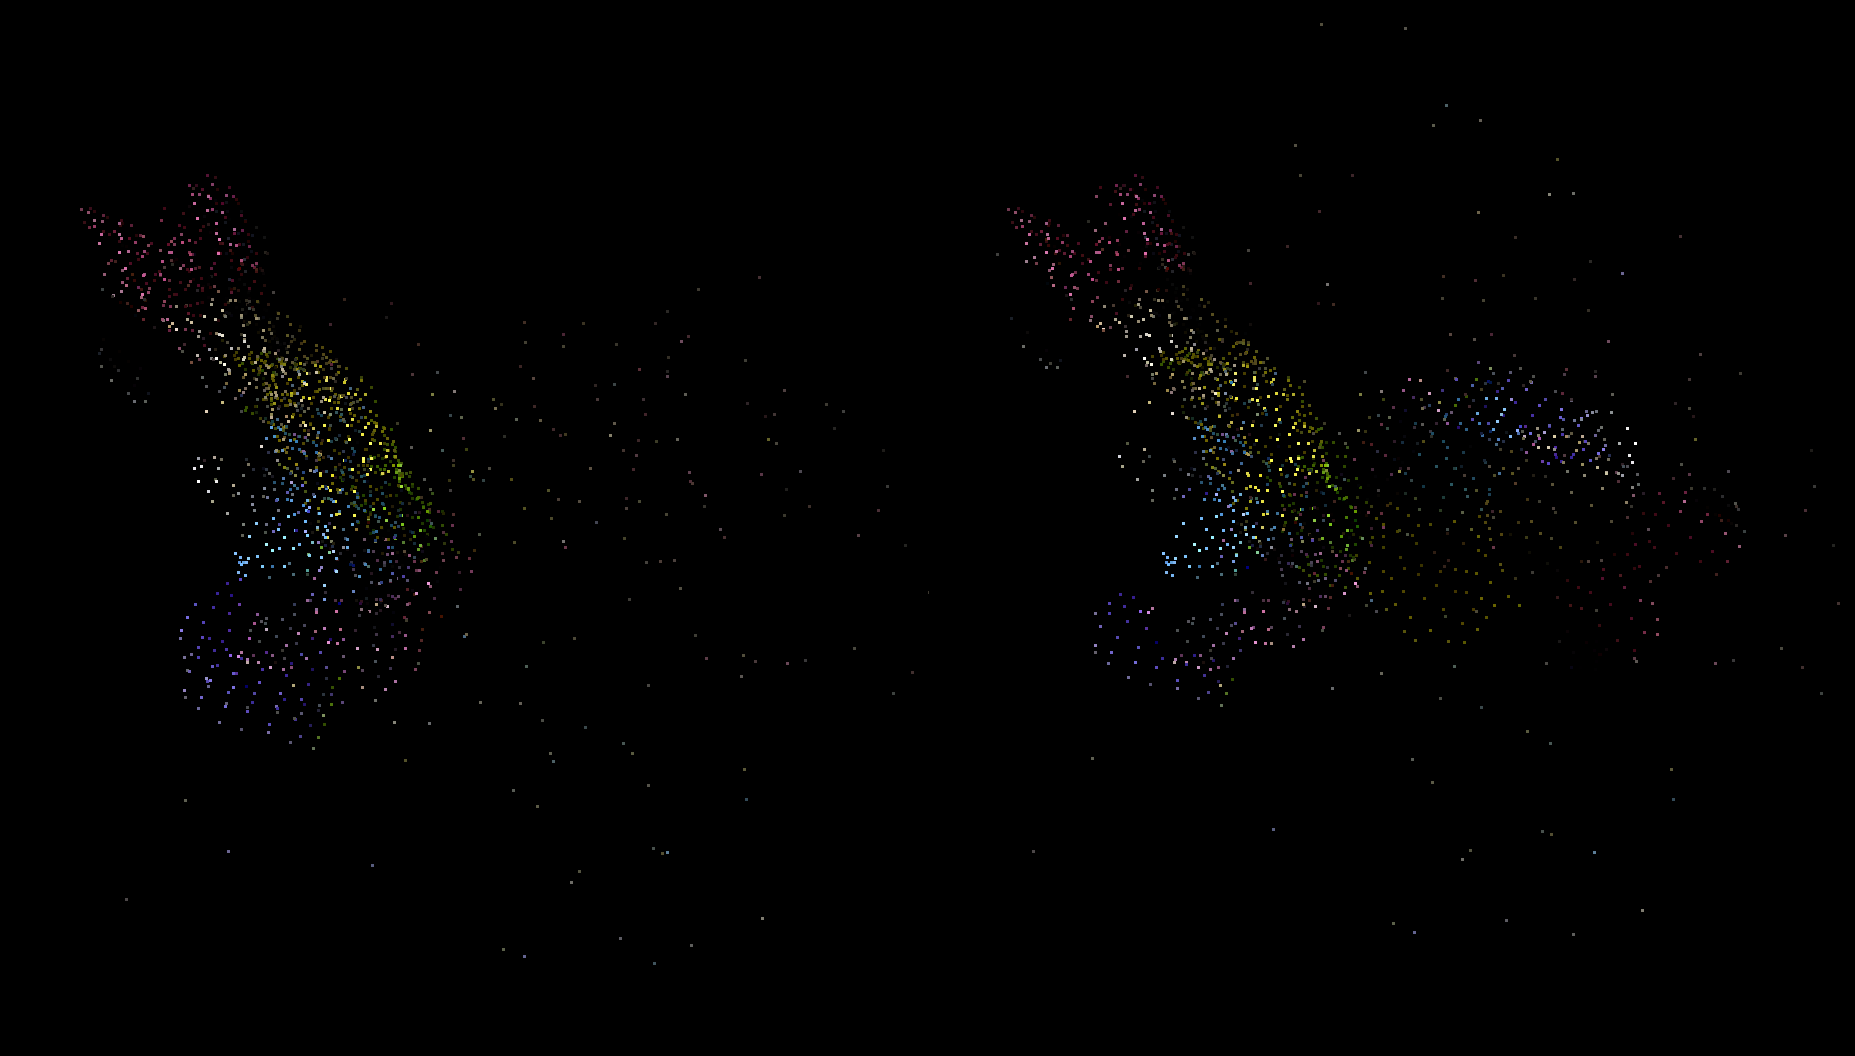
\includegraphics[width=1\textwidth]{images/lab3.png}
		\caption{\label{fig:lab3}Due metodi di registrazione a confronto.}
	\end{figure}


\section{Lab 4} \label{sec:lab4}
La quarta esperienza richiedeva di mettere insieme le tecniche aquisite nelle tre precedenti per registrare tra loro delle point cloud di un robot Nao riprese in scene di media complessità. In preparazione a questo è stato svolto un esercizio che richiedeva di modificare un people detector preesitente in modo che non richiedesse input da parte dell'utente. Il people detector, per identificare correttamente le persone, deve individuare come prima cosa il pavimento; è stato quindi aggiunto al codice una stima automatica del ground plane.\\
La registrazione del Nao ha richiesto più passaggi:
\begin{itemize}
	\item stima e rimozione del ground plane;
	\item rimozione dello sfondo;
	\item identificazione dei keypoint;
	\item estrazione dei descrittori;
	\item stima delle corrispondenze;
	\item registrazione;
\end{itemize}


	\subsection{Algortimi utilizzati}


	\subsection{Considerazioni}


\begin{thebibliography}{9}
\bibitem{nano3}
  K. Grove-Rasmussen og Jesper Nygård,
  \emph{Kvantefænomener i Nanosystemer}.
  Niels Bohr Institute \& Nano-Science Center, Københavns Universitet

\end{thebibliography}
\end{document}